% Author:Yuya Aoki
\documentclass{jsarticle}
\usepackage{graphicx}
\usepackage{booktabs}
\title{巡回セールスマン問題}
\author{1776002 青木裕哉}
\date{2017/11/20}
\begin{document}
\fontsize{10pt}{12pt}\selectfont
\maketitle

\section{課題1 全探索}
\begin{table}
  \centering
	\begin{tabular}[p]{ccc}
		\toprule
		citys & range & time \\
		5 & 2.364416 & 0.00001600000000 sec \\
		10 & 3.069126 & 0.05755400000000 sec \\
		11 & 2.994373 & 0.67660700000000 sec \\
		12 & 3.019338 & 7.81969200000000 sec \\
		13 & 3.281921 & 99.89479900000001 sec \\
		\bottomrule
	\end{tabular}
	\caption{全探索による回答と計算時間}
\end{table}


\section{課題2 改善法}
\begin{table}
  \centering
	\begin{tabular}[p]{ccc}
		\toprule
		citys & true & improved \\
		5  & 0.00001600000000 sec  &  0.01858900000000 sec \\
		10 & 0.05755400000000 sec  &  0.02077800000000 sec \\
		11 & 0.67660700000000 sec  &  0.02763800000000 sec \\
		12 & 7.81969200000000 sec  &  0.03142700000000 sec \\
		13 & 99.89479900000001 sec &  0.03948900000000 sec \\
		\bottomrule
	\end{tabular}
	  \caption{改善法と全探索における計算時間の比較}
\end{table}

配布されていた全探索のコードは
$O(n!)$ ほどの計算量だった.
改善法は完全にランダムのため計算量は一定でないが,
局所解に収束しやすいため,非常に少ない計算量になった.
今回のプログラムでは,
解の精度向上のため,
100000回試行して改善されなかったという条件を計算の終了とした.
そのため,計算量の理想値である
$O(n^2)$
ではなく,最大で
$O(100000 + 2 \times n^2)$
程度の計算量となった.
以下のプログラムでも同様の条件を計算の終了条件としている.

\section{課題3 構築法}
計算量は必ず
$O(n \times (n - 1) )$
となるが,局所解に陥り安く,精度は損なわれる.
具体的には以下の図の通りである.


\begin{figure}[htb]
  \centering
    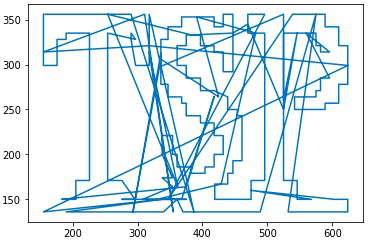
\includegraphics[width=1cm]{CM225.png}
	\caption{構築法による225都市の巡回セールスマン問題の解答}
\end{figure}

\section{課題4 アニーリング法}



\end{document}


